\documentclass[dvipsnames,hidelinks,t]{beamer}

  % Enables the use of colour. 
  \usepackage{xcolor}
  % Syntax high-lighting for code. Requires Python's pygments.
  \usepackage{minted}
  % Enables the use of umlauts and other accents.
  \usepackage[utf8]{inputenc}
  % Diagrams.
  \usepackage{tikz}
  % Settings for captions, such as sideways captions.
  \usepackage{caption}
  % Symbols for units, like degrees and ohms.
  \usepackage{gensymb}
  % Latin modern fonts - better looking than the defaults.
  \usepackage{lmodern}
  % Allows for columns spanning multiple rows in tables.
  \usepackage{multirow}
  % Better looking tables, including nicer borders.
  \usepackage{booktabs}
  % More math symbols.
  \usepackage{amssymb}
  % More math fonts, like mathbb.
  \usepackage{amsfonts}
  % More math layouts, equation arrays, etc.
  \usepackage{amsmath}
  % More theorem environments.
  \usepackage{amsthm}
  % More column formats for tables.
  \usepackage{array}
  % Adjust the sizes of box environments.
  \usepackage{adjustbox}
  % Better looking single quotes in verbatim and minted environments.
  \usepackage{upquote}
  % Better blank space decisions.
  \usepackage{xspace}
  % Better looking tikz trees.
  \usepackage{forest}
  % URLs.
  \usepackage{hyperref}
  % For plotting.
  \usepackage{pgfplots}
  
  % Various tikz libraries.
  % For drawing mind maps.
  \usetikzlibrary{mindmap}
  % For adding shadows.
  \usetikzlibrary{shadows}
  % Extra arrows tips.
  \usetikzlibrary{arrows.meta}
  % Old arrows.
  \usetikzlibrary{arrows}
  % Automata.
  \usetikzlibrary{automata}
  % For more positioning options.
  \usetikzlibrary{positioning}
  % Creating chains of nodes on a line.
  \usetikzlibrary{chains}
  % Fitting node to contain set of coordinates.
  \usetikzlibrary{fit}
  % Extra shapes for drawing.
  \usetikzlibrary{shapes}
  % For markings on paths.
  \usetikzlibrary{decorations.markings}
  % For advanced calculations.
  \usetikzlibrary{calc}
  
  % GMIT colours.
  \definecolor{gmitblue}{RGB}{20,134,225}
  \definecolor{gmitred}{RGB}{220,20,60}
  \definecolor{gmitgrey}{RGB}{67,67,67}
  
  % Change some style options.
  \usetheme{metropolis}
  % Tell minted to use the following colour scheme. 
  \usemintedstyle{manni}
  % Remove some of the vertical space after the title.
  \addtobeamertemplate{frametitle}{}{\vspace{-3mm}}
  % Change the default theme colours.
  \setbeamercolor{normal text}{fg=darkgray, bg=white}
  \setbeamercolor{alerted text}{fg=gmitred, bg=white}
  \setbeamercolor{example text}{fg=gmitblue, bg=white}
  \setbeamercolor{frametitle}{fg=gmitblue, bg=white}
  \setbeamercolor*{item}{fg=gmitblue}
  % Use a better math mode font.
  \usefonttheme[onlymath]{serif}
  % Don't display section pages.
  \metroset{sectionpage=none}
  % Change the default itemize bullets.
  \setbeamertemplate{itemize item}{\color{gray}--}
  % Change the position of left aligned math.
  %\setlength{\mathindent}{7mm}

  % An environment for displaying math in red, without lots of vertical space.
  \newcommand{\redmath}[1]{\vspace{-3mm} {\begin{center} \color{gmitred} $ #1 $ \end{center}} \vspace{-2mm}}

  % For displaying a blank character.
  \newcommand{\bl}{\underline{\hspace{2mm}}}

  % \citeurl can be used to a clickable short url to a slide as a reference.
  \renewcommand\footnoterule{}
  \newcommand{\citeurl}[1]{\let\thefootnote\relax\footnotetext{\tiny \textcolor{gmitgrey}{\href{http://#1}{#1}}}}
  \newcommand{\citeeg}[1]{\let\thefootnote\relax\footnotetext{\tiny \textcolor{gmitgrey}{#1}}}
  
  % Prevent minted from showing errors.
  \makeatletter
  \expandafter\def\csname PYGdefault@tok@err\endcsname{\def\PYGdefault@bc##1{{\strut ##1}}}
  \makeatother
  
  \begin{document}
    \title{Graph isomorphisms}
    \subtitle{}
    \author{ian.mcloughlin@gmit.ie}
    \date{}
  
    \begin{frame}
      \titlepage
    \end{frame}
  
    \begin{frame}{Bijections}
  
  A bijection is map $f$ from a set $X$ to a set $Y$ where both of the following are true:
  \begin{itemize}
    \item every $y$ in $Y$ is a value $f(x)$ for at most one $x$ in $X$.
    \item every $y$ in $Y$ is a value $f(x)$ for at least one $x$ in $X$.
  \end{itemize}
  
  \begin{center}
    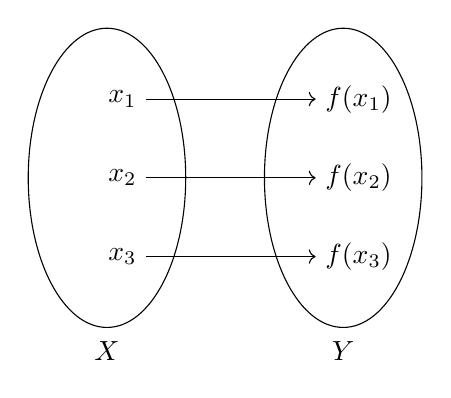
\begin{tikzpicture}
      \draw (0,0) ellipse (1 and 1.9);
      \draw (0,-2.2) node {$X$};
      \draw (3,0) ellipse (1 and 1.9);
      \draw (3,-2.2) node {$Y$};

      \draw [->]  (0.5,1) node[anchor=east] {$x_1$} -- (2.65,1) node[anchor=west] {$f(x_1)$};
      \draw [->]  (0.5,0) node[anchor=east] {$x_2$} -- (2.65,0) node[anchor=west] {$f(x_2)$};
      \draw [->]  (0.5,-1) node[anchor=east] {$x_3$} -- (2.65,-1) node[anchor=west] {$f(x_3)$};
    \end{tikzpicture}
  \end{center}
  
\end{frame}
  
  
\begin{frame}{Isomorphisms}
  \begin{itemize}
    \item Two graphs $G_1 = (V_1,E_1)$ and $G_2=(V_2,E_2)$ are said to be isomorphic when there is a bijection $f$ from $V_1$ to $V_2$ Bsuch that $\{f(x), f(y) \}$ is in $E_2$ if and only if $(x,y)$ is in $E_1$.
    \item Then $f$ is said to be an isomorphism.
    \item So, an isomorphism is a bijection between the vertex sets that preserves the edges.
  \end{itemize}
  \vspace{4mm}
  \begin{center}
    \begin{columns}
      \begin{column}{0.3\textwidth}
        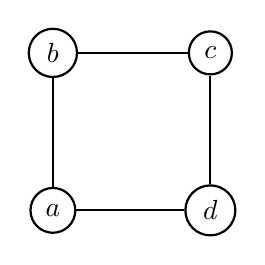
\begin{tikzpicture}
          \begin{scope}[every node/.style={circle,thick,draw}]
            \node (a) at (0,0) {$a$};
            \node (b) at (0,2) {$b$};
            \node (c) at (2,2) {$c$};
            \node (d) at (2,0) {$d$};
          \end{scope}
          \begin{scope}[every edge/.style={draw=black,thick}]
            \path (a) edge (b);
            \path (b) edge (c);
            \path (c) edge (d);
            \path (d) edge (a);
          \end{scope}
        \end{tikzpicture}
      \end{column}
      
      \begin{column}{0.3\textwidth}
        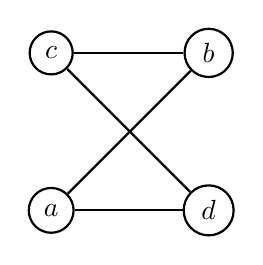
\begin{tikzpicture}
          \begin{scope}[every node/.style={circle,thick,draw}]
            \node (a) at (0,0) {$a$};
            \node (c) at (0,2) {$c$};
            \node (b) at (2,2) {$b$};
            \node (d) at (2,0) {$d$};
          \end{scope}
          \begin{scope}[every edge/.style={draw=black,thick}]
            \path (b) edge (c);
            \path (c) edge (d);
            \path (b) edge (a);
            \path (d) edge (a);
          \end{scope}
        \end{tikzpicture}
      \end{column}
      
      \begin{column}{0.3\textwidth}
        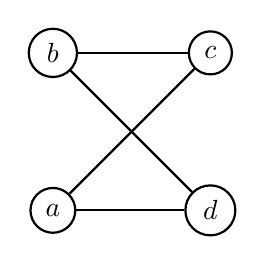
\begin{tikzpicture}
          \begin{scope}[every node/.style={circle,thick,draw}]
            \node (a) at (0,0) {$a$};
            \node (b) at (0,2) {$b$};
            \node (c) at (2,2) {$c$};
            \node (d) at (2,0) {$d$};
          \end{scope}
          \begin{scope}[every edge/.style={draw=black,thick}]
            \path (b) edge (c);
            \path (b) edge (d);
            \path (c) edge (a);
            \path (d) edge (a);
          \end{scope}
        \end{tikzpicture}
      \end{column}
    \end{columns}
  \end{center}
  
\end{frame}
  
  
\begin{frame}{Isomorphism example}
  \begin{center}
    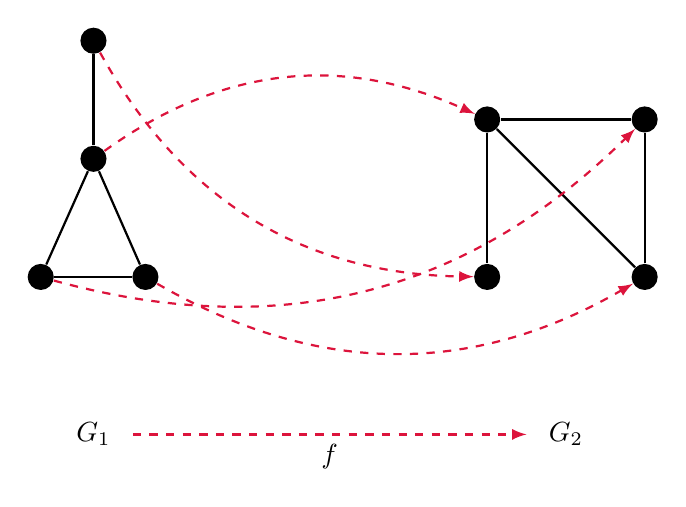
\begin{tikzpicture}
      \begin{scope}[every node/.style={circle, fill=black}]
        \node (a) at (1   ,1.5) {};
        \node (b) at (1   ,3) {};
        \node (c) at (0.33,0) {};
        \node (d) at (1.66,0) {};
      \end{scope}
      \begin{scope}[every edge/.style={draw=black,thick}]
        \path (a) edge (b);
        \path (a) edge (c);
        \path (a) edge (d);
        \path (c) edge (d);
      \end{scope}
      \begin{scope}[every node/.style={circle, fill=black}]
        \node (1) at (6,2) {};
        \node (2) at (6,0) {};
        \node (3) at (8,2) {};
        \node (4) at (8,0) {};
      \end{scope}
      \begin{scope}[every edge/.style={draw=black,thick}]
        \path (1) edge (2);
        \path (1) edge (3);
        \path (1) edge (4);
        \path (3) edge (4);
      \end{scope}
      \begin{scope}[every edge/.style={draw=gmitred, dashed, thick, ->, >=latex}]
        \path (a) edge[bend left] (1);
        \path (b) edge[bend right] (2);
        \path (c) edge[bend right] (3);
        \path (d) edge[bend right] (4);
      \end{scope}
      \node at (1,-2) {$G_1$};
      \node at (7,-2) {$G_2$};
      \path (1.5,-2) edge[draw=gmitred, dashed, thick, ->, >=latex] node[below] {$f$} (6.5,-2);
    \end{tikzpicture}
  \end{center}
\end{frame}
  
\begin{frame}{Exercise}
  
  Determine if these two graphs are isomorphic.
  
  \begin{columns}
    \begin{column}{0.5\textwidth}
      \begin{center}
        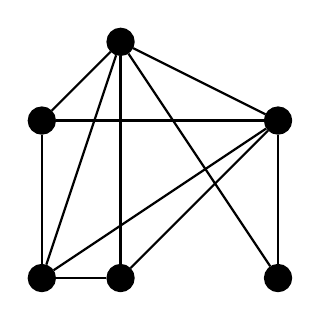
\begin{tikzpicture}
          \begin{scope}[every node/.style={circle,thick,draw,fill}]
            \node (a) at (0,1) {};
            \node (b) at (0,4) {};
            \node (c) at (2,1) {};
            \node (d) at (2,3) {};
            \node (e) at (-1,1) {};
            \node (f) at (-1,3) {};
          \end{scope}
          \begin{scope}[every edge/.style={draw=black,thick}]
            \path (a) edge (b);
            \path (a) edge (d);
            \path (a) edge (e);
            \path (b) edge (c);
            \path (b) edge (d);
              \path (b) edge (e);
              \path (b) edge (f);
              \path (c) edge (d);
              \path (d) edge (e);           
              \path (d) edge (f);
              \path (e) edge (f);
          \end{scope}
        \end{tikzpicture}
      \end{center}
    \end{column}
    \begin{column}{0.5\textwidth}
      \vspace{10mm}
      \begin{center}
        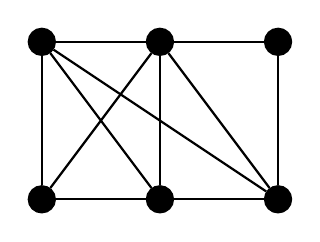
\begin{tikzpicture}
          \begin{scope}[every node/.style={circle,fill,thick,draw}]
            \node (a) at (0,0) {};
            \node (b) at (0,2) {};
            \node (c) at (1.5,0) {};
            \node (d) at (1.5,2) {};
            \node (e) at (3,0) {};
            \node (f) at (3,2) {};
          \end{scope}
          \begin{scope}[every edge/.style={draw=black,thick}]
            \path (a) edge (b);
            \path (a) edge (c);
            \path (c) edge (e);
            \path (a) edge (d);
            \path (b) edge (c);
            \path (b) edge (d);
              \path (b) edge (e);
              \path (b) edge (d);
              \path (d) edge (f);
              \path (c) edge (d);
              \path (d) edge (e);	            
              \path (e) edge (f);
          \end{scope}
        \end{tikzpicture}
      \end{center}
    \end{column}
  \end{columns}
\end{frame} 
  \end{document}